\documentclass[10pt,sigconf]{acmart}
\synctex=1
\graphicspath{{figures/}{doc/paper/}}
\usepackage[l2tabu,orthodox]{nag}
\usepackage[utf8x]{inputenc}
\usepackage[british]{babel}
\usepackage{microtype}
\usepackage[caption=false]{subfig}
\usepackage{graphicx}
\usepackage{url}
\usepackage{color}

\frenchspacing
\uchyph=0

\newcommand{\todo}[1]{\textbf{\textcolor{red}{To do: #1}}}
\newcommand{\idea}[1]{{\textcolor{blue}{#1}}}

%==================================================================================================
\begin{document}
\title{Does TCP New Congestion Window Validation Improve HTTP Adaptive Streaming Performance?}

\author{Mihail Yanev}
    \orcid{0000-0002-9814-1017}
    \affiliation{
      \institution{University of Glasgow}
      \streetaddress{School of Computing Science}
      \city{Glasgow}
      \postcode{G12 8QQ}
      \country{UK}
    }
    \email{m.yanev.1@research.gla.ac.uk}

  \author{Stephen McQuistin}
    \orcid{0000-0002-0616-2532}
    \affiliation{
    \institution{University of Glasgow}
    \streetaddress{School of Computing Science}
    \city{Glasgow}
    \postcode{G12 8QQ}
    \country{UK}
    }
    \email{sm@smcquistin.uk}

\author{Colin Perkins}
  \orcid{0000-0002-3404-8964}
  \affiliation{
    \institution{University of Glasgow}
    \streetaddress{School of Computing Science}
    \city{Glasgow}
    \postcode{G12 8QQ}
    \country{UK}
  }
  \email{csp@csperkins.org}

\copyrightyear{2022}
\acmYear{2022}
\setcopyright{acmlicensed}
\acmConference[NOSSDAV'22]{The 32nd edition of
  the Workshop on Network and Operating System Support for Digital Audio and
  Video}{June 17, 2022}{Athlone, Ireland}
\acmBooktitle{The 32nd edition of the Workshop on Network and Operating
  System Support for Digital Audio and Video (NOSSDAV'22), June 17, 2022,
  Athlone, Ireland}
\acmPrice{15.00}
\acmDOI{10.1145/3534088.3534347}
\acmISBN{978-1-4503-9383-6/22/06}

\begin{CCSXML}
<ccs2012>
   <concept>
       <concept_id>10003033.10003039.10003048</concept_id>
       <concept_desc>Networks~Transport protocols</concept_desc>
       <concept_significance>300</concept_significance>
       </concept>
   <concept>
       <concept_id>10003033.10003039.10003051</concept_id>
       <concept_desc>Networks~Application layer protocols</concept_desc>
       <concept_significance>300</concept_significance>
       </concept>
   <concept>
       <concept_id>10003033.10003079.10003081</concept_id>
       <concept_desc>Networks~Network simulations</concept_desc>
       <concept_significance>100</concept_significance>
       </concept>
   <concept>
       <concept_id>10003033.10003068.10003073.10003075</concept_id>
       <concept_desc>Networks~Network control algorithms</concept_desc>
       <concept_significance>500</concept_significance>
       </concept>
 </ccs2012>
\end{CCSXML}

\ccsdesc[300]{Networks~Transport protocols}
\ccsdesc[300]{Networks~Application layer protocols}
\ccsdesc[100]{Networks~Network simulations}
\ccsdesc[500]{Networks~Network control algorithms}

%==================================================================================================
\begin{abstract}

  
  % Four sentences:
  %  - State the problem
  %  - Say why it's an interesting problem
  %  - Say what your solution achieves
  %  - Say what follows from your solution

When using HTTP adaptive streaming, video traffic exhibits on-off behaviour with frequent idle periods that can interact poorly with TCP congestion control algorithms. New congestion window validation (New CWV) modifies TCP to allow senders to restart more quickly after certain idle periods. While previous work has shown that New CWV can improve \emph{transport} performance for streaming video, it remains to demonstrate that this translates to improved \emph{application} level performance, in terms of playback stability. In this paper, we show that enabling New CWV can reduce video re-buffering events by up to 4\%, and limit representation switches by 12\%, without any changes to existing rate adaptation algorithms.

\end{abstract}
\maketitle
%==================================================================================================
\section{Introduction}
\label{sec:introduction}

Video streaming over HTTP is commonplace, and comprises the majority of Internet traffic~\cite{Sandvine-2019-global-internet-report}. The performance of such HTTP adaptive streaming video is generally very good, and gives a high-quality user experience.
  
There are, however, some scenarios where HTTP adaptive streaming can perform comparatively poorly \cite{Spiteri-2016-BOLA,Kua-2017-a-survey-rate-adaptation-dash}. In particular, the interaction between the on-off traffic patterns generated by adaptive streaming applications and TCP congestion control algorithms can reduce the performance of throughput-based video rate adaptation schemes~\cite{Akhshabi-2012-http-adaptive-players-compete,Stohr-2017-where-are-the-sweet-spots-maci}. In some cases, this is due to the TCP congestion window validation (CWV)~\cite{rfc2861-2000-padhye-congestion-window-validation} algorithm that, while preventing TCP clients from sending using stale knowledge of the network, has been shown to negatively impact the throughput of rate-limited applications~\cite{Nazir-2014-performance-evaluation-congestion-window-validation-dash-newcwv}, including HTTP adaptive streaming. New congestion window validation (New CWV)~\cite{rfc7661-2015-fairhurst-new-cwnd-validation} has been proposed to address this. Prior work~\cite{Nazir-2014-performance-evaluation-congestion-window-validation-dash-newcwv} has demonstrated that New CWV has the desired \emph{transport} layer impact, but it remains to show that this translates to improved quality of experience (QoE) performance at the \emph{application} layer. This is not guaranteed, given the complexity that exists at both layers, and that results from their interaction. For example, large discrepancies between video bandwidth requirements and the available link capacity, or the requirement for stable, long-lived connections in modern streaming video players can influence rate adaptation~\cite{Spiteri-2019-from-theory-to-practice-sabre}.

In this paper, we investigate whether enabling New CWV improves video playback stability and, more generally, video QoE for HTTP adaptive streaming over TCP. We compare video performance using TCP New Reno with the CWV and New CWV algorithms. We collect standard video performance metrics, including bit-rate oscillation, and stall time, to measure stability and QoE. Further, to quantify the impact of New CWV with respect to the inferred network state at the client, we also record the immediate and smoothened client's link capacity estimations for each delivered chunk.

In particular, we make the following contributions: (i) an implementation of New CWV for Linux (kernel version 5.4); (ii) a testbed setup for evaluating New CWV's application layer impact; and (iii) results that demonstrate that New CWV improves video stability, with a 12\% reduction in bit rate switches, and a 4\% reduction in rebuffering time.


To the best of our knowledge, this is the first paper to study the application
layer impact of enabling New CWV. 
Nazir et al. \cite{Nazir-2014-performance-evaluation-congestion-window-validation-dash-newcwv}
demonstrated the effect of New CWV on the transport layer, and there has been a large amount of work that has proposed new application layer rate adaptation algorithms~\cite{Mok-2012-qdash,Huang-2015-A-buffer-based-approach-to-rate-adaptation-bba, Yin-2015-a-control-theoritic-approach}. In contrast, we only change the transport algorithm, and leave the application as is, studying the transport's impact on the application. Improving performance via transport layer modifications could allow for simpler rate adaptation algorithms at the application layer.


We structure the remainder of this paper as follows. In Section~\ref{sec:background}, we introduce TCP congestion window validation, including its limitations with respect to HTTP adaptive video flows, before describing New CWV. Section~\ref{sec:evaluation} describes our experimental setup, and the transport and application layer impact of enabling New CWV. Section~\ref{sec:related} describes related work, and Section~\ref{sec:conclusion} concludes.

%==================================================================================================
\section{Congestion Window Validation}
\label{sec:background}

\begin{figure}
  \centering
    \subfloat[CWV]{
      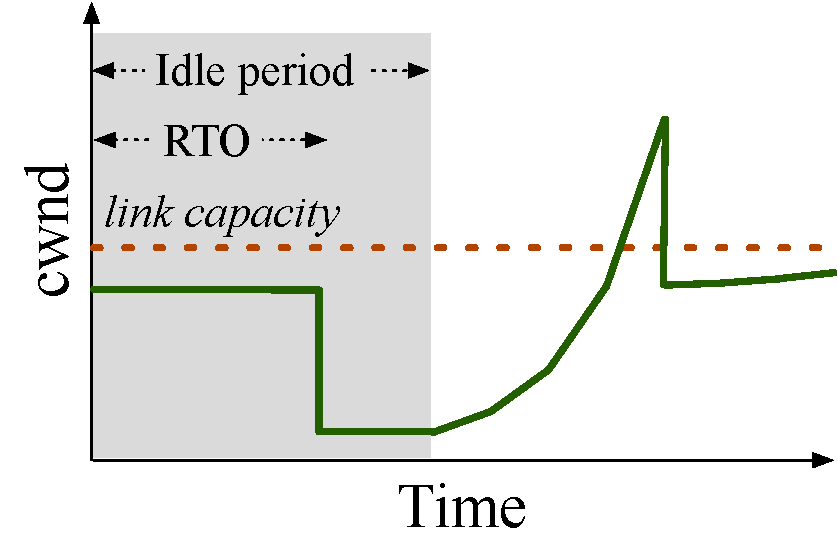
\includegraphics[width=.23\textwidth]{figures/cwv.pdf}
      \label{fig:cwv}
    }
    \subfloat[New CWV]{
      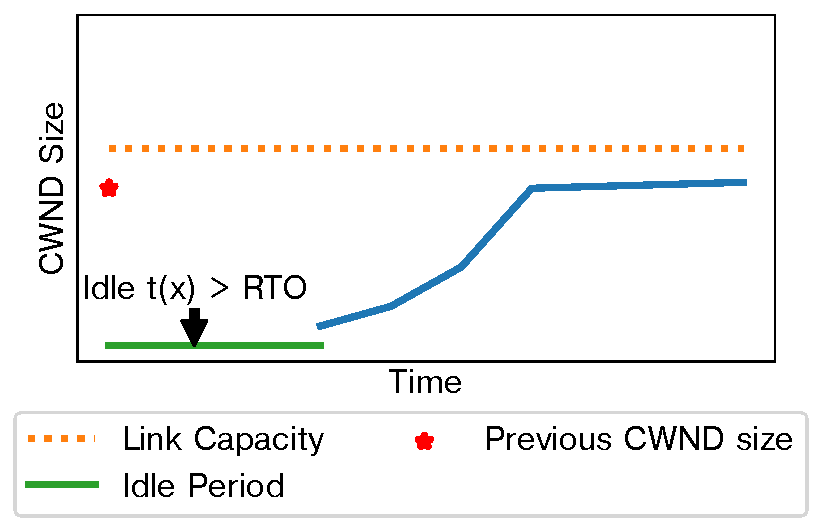
\includegraphics[width=.23\textwidth,]{figures/new_cwv.pdf}
      \label{fig:newcwv}
    }
    \caption{Illustration of \emph{cwnd} growth following an idle period}
    \label{fig:cwnd-growth-after-idle}
\end{figure}

In HTTP adaptive streaming, a server provides pre-encoded video chunks in different representations, each encoded at multiple bit rates, while the client, using a rate adaptation algorithm, determines the best representation to request at any given time. The goal of the client is to maximise QoE within the network's capacity. This can be a challenge since different, often contradictory, QoE heuristics need be considered simultaneously~\cite{Seufert-2015-A-Survey-on-QoE-Dash}. 

Throughput-based rate adaptation algorithms for HTTP adaptive streaming use an estimate of the current network conditions to determine the representation that should be requested. These algorithms require a stable and accurate throughput estimate in order to perform well. However, the interaction between the on-off traffic pattern of streaming video and TCP's congestion control algorithm can lead to significant fluctuations in throughput, impacting the performance of throughput-based rate adaptation algorithms.


In particular, during idle periods in between transmission of video chunks, the TCP congestion controller's knowledge of the network capacity becomes stale. To avoid sending with a possibly unrepresentative congestion window, once the link has been idle for a period longer than the connection's retransmission timeout, $T_{rto}$, the congestion window validation~\cite{rfc2861-2000-padhye-congestion-window-validation} (CWV) algorithm resets the TCP congestion window (\emph{cwnd}) to its initial value and forces the connection to re-enter slow-start after an idle period. Figure~\ref{fig:cwv} illustrates the behaviour of CWV following an idle period. CWV has become standard practice~\cite{rfc5681-congeston-control}, and is enabled by default in the latest stable Linux kernel (5.4). However, re-entering slow-start like this, results in packet loss once the CWND grows beyond the link capacity (Figure~\ref{fig:transmission-after-idle-reno}). This was found to interact poorly with HTTP adaptive streaming and other application-limited transmissions~\cite{Esteban-2012-Interactions-HTTP-TCP}.

To address re-entering slow start, new congestion window validation~\cite{rfc7661-2015-fairhurst-new-cwnd-validation} was proposed. During a slow-start after idle rather than relying on packet loss to re-discover its appropriate \emph{cwnd} value, New CWV preserves the \emph{cwnd} before the idle period and later uses it as a slow-start threshold (\emph{ssthresh}), i.e., it to exit the slow-start phase earlier, before loss occurs. Figure~\ref{fig:newcwv} shows the growth of \emph{cwnd} following an idle period under New CWV.

\begin{figure}[t!]
  \centering
  \subfloat[CWV]{
    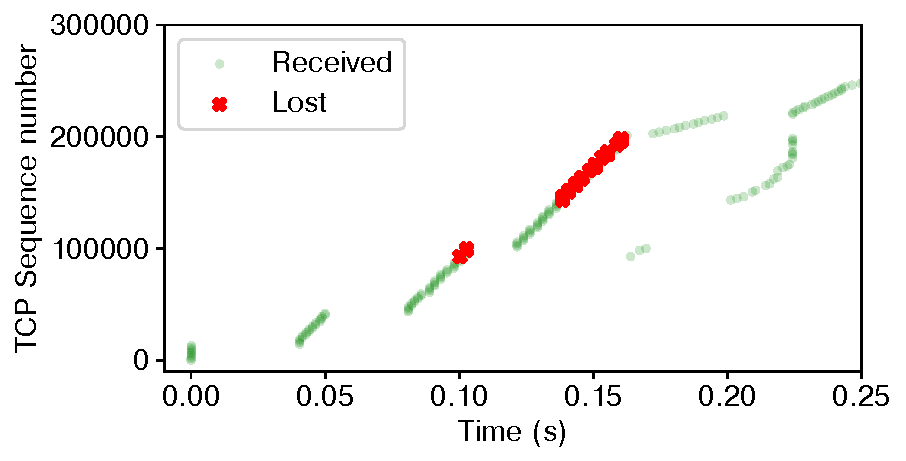
\includegraphics[width=.45\textwidth, keepaspectratio]{figures/lost_packets_vreno.pdf}
    \label{fig:transmission-after-idle-reno}
  }
  \\
    \subfloat[New CWV]{
      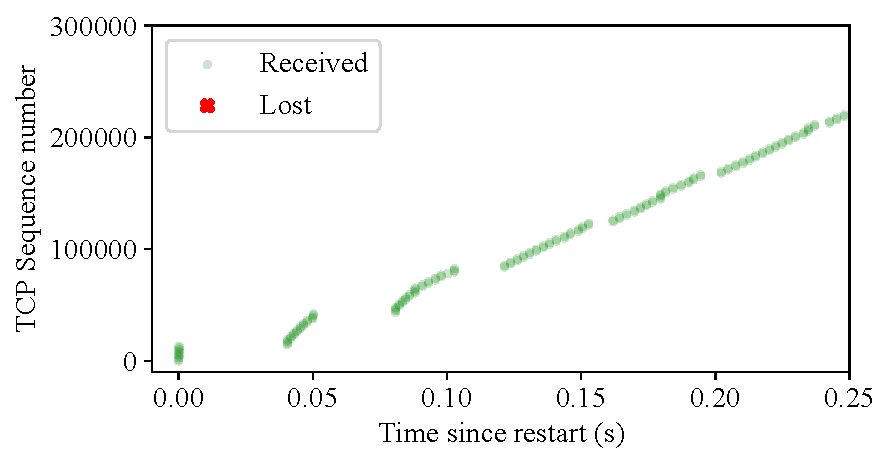
\includegraphics[width=.45\textwidth, keepaspectratio]{figures/lost_packets_newcwv.pdf}
      \label{fig:transmission-after-idle-newcwv}
    }
    \caption{Resumption after an idle period}
    \label{fig:transmission-after-idle}
\end{figure}

To evaluate the transport performance of New CWV, we have implemented the algorithm within the Linux kernel~\footnote{A snapshot of our implementation, as used in this paper, is available at \url{http://dx.doi.org/10.5525/gla.researchdata.1278}, while the main repository for the work is at \url{https://github.com/glasgow-ipl/newcwv-nossdav2022}.}. We used \cite{secchi-2016-newcwv} as a base, which provides a Kernel 3.18 implementation. Our implementation altered two files adding 143 and removing 49 lines of code. We use this implementation to better illustrated the impact of New CWV on flows restarting after an idle period, as shown in Figure~\ref{fig:transmission-after-idle}.
As shown, the connection using New CWV uses the previously set \emph{ssthresh} value and leaves slow-start early. This results in New CWV connections not experiencing any packet loss (Figure~\ref{fig:transmission-after-idle-newcwv}), after reaching their set \emph{ssthresh} value in the third flight of packets after restarting. In contrast, if the same connection used CWV, the senders would not have preserved the \emph{ssthresh} value that way and would rely on loss to exit slow-start, as seen at the end of the third and fourth flights of packets in Figure~\ref{fig:transmission-after-idle-reno}. In the presented case, CWV enters congestion avoidance around 160 milliseconds after the transmission restart (Figure \ref{fig:transmission-after-idle-reno}), while New CWV is able to enter congestion avoidance around the 110th millisecond mark (Figure \ref{fig:transmission-after-idle-newcwv}).

Overall, New CWV results in fewer lost packets, and returns to its previous sending rate without overshoot after loss, giving more predictable transmission.

New CWV has been shown to improve \emph{transport} layer performance of rate-limited applications when compared with CWV~\cite{Nazir-2014-performance-evaluation-congestion-window-validation-dash-newcwv}, and our implementation and the results we have presented here validate that. It remains to show how this translates into \emph{application} layer performance, particularly since this is not guaranteed~\cite{Spiteri-2016-BOLA}. In Section~\ref{sec:evaluation}, we first validate the results of Nazir et al.~\cite{Nazir-2014-performance-evaluation-congestion-window-validation-dash-newcwv}, before testing our hypothesis that New CWV will enable applications to obtain more consistent throughput estimates, and, in turn, improve the stability of throughput-based rate adaptation algorithms.

%==================================================================================================
\section{Evaluating New CWV for Video}
\label{sec:evaluation}

\begin{figure}
  \centering
  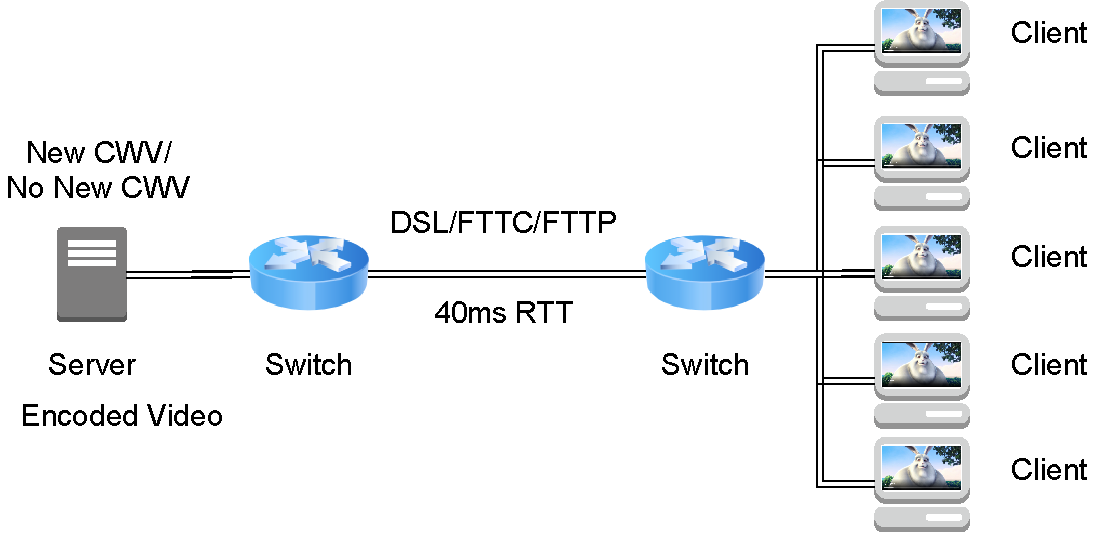
\includegraphics[width=.45\textwidth]{figures/setup.pdf}
  \caption{Experimental Setup}
  \label{fig:experimental-setup}
\end{figure}

We first describe our experimental setup (\S\ref{sec:experimental-setup}), which we use to investigate the transport layer impact, verify whether New CWV connections obtain more consistent throughput estimates (\S\ref{sec:transport-impact}), and later to also investigate the application impact, and more specifically, the difference on video QoE that New CWV connections observe (\S\ref{sec:QoE-impact}). Finally, we summarise our findings (\S\ref{sec:summary}).

%--------------------------------------------------------------------------------------------------
\subsection{Experimental Setup}
\label{sec:experimental-setup}

% Overview
Our evaluation testbed consists of a network emulated in Mininet, running on Ubuntu 20.04, as shown in Figure~\ref{fig:experimental-setup}. Both the server and its clients use TCP New Reno and run Linux Kernel 5.4.0 modified to include New CWV and RFC 3339~\cite{rfc3339-precise-timestamps} compliant timestamps to enable higher precision event tracking. 

% Server
The server uses \texttt{nginx} (v1.18) with HTTP/2, serving three representations of Big Buck Bunny\footnote{\url{https://download.blender.org/demo/movies/BBB/}}: 480p (0.44Mbps), 720p (2.64Mbps), and 1080p (4.82Mbps). Each is encoded in chunks of 3 seconds duration.
%  Client
Clients use Firefox (v91) with \texttt{dash.js}\footnote{\url{https://github.com/Dash-Industry-Forum/dash.js}} (v4.0.0). We
report results with both the \textsc{throughput} and \textsc{dynamic} \cite{Spiteri-2019-from-theory-to-practice-sabre} algorithms implemented in \texttt{dash.js}.

The network is configured with a bottleneck RTT of 40ms, a reasonable RTT value to the closest video CDN replica. The routers' queues are sized to the bandwidth delay product. Three different bandwidth profiles are evaluated, representing DSLv2 (10Mbps), FTTC (50Mbps), and FTTP (145Mbps) links; e.g., as are typical in the UK~\cite{ofcom-2020-report}. Below we show the results for the DSLv2 and FTTC links. While FTTP links are deployed in some regions we note that DSLv2 and FTTC links are still common~\cite{ofcom-2020-report, FCC-measuring-broadband-america, EC-measuring-broadband-europe, ACCC-measuring-broadband-australia}. As higher resolution video and other network-heavy operations such as virtual reality environments become more available we expect the issues observed could translate to the links with higher capacity (i.e., FTTC and FTTP).

As our experiments investigate the effect of New CWV when only video traffic is present, the chosen homogeneous RTT value fits our experiment design, since in practice, traffic for such scenarios would likely come from the same streaming server or CDN replica.

We leave as future work the creation of a more complex environment, e.g., video clients starting at random times, evaluating New CWV performance when it interacts with clients in all TCP states, introducing non-homogenous traffic and cross traffic, inspecting how video controlled New CWV flows interact with other types of traffic, etc.   

To evaluate the impact of congestion and competing flows, experiments were run with both the \textsc{dynamic} and \textsc{throughput} algorithms and several (1, 2, 3, and 5) simultaneous clients. Finally, to reduce noise, we ran each combination of CWV or New CWV, adaptive algorithm, number of clients, and link type, 10 times before reporting the average results. The results presented includes data accumulated from 480 simulations (2 congestion control algorithms $\times$ 2 adaptive algorithms $\times$ 3 link types $\times$ 4 client variations $\times$ 10 repetitions). 
During each run we collect client bandwidth estimates. Additionally, to evaluate the video QoE impact we report the rebuffer ratio and bitrate switch frequency distribution.

%--------------------------------------------------------------------------------------------------
\subsection{Impact on Transport Performance} 
\label{sec:transport-impact}

New CWV alters the TCP \emph{cwnd} sizing behaviour, allowing it to recover more quickly after an idle period. As shown in Figures~\ref{fig:newcwv} and \ref{fig:transmission-after-idle-newcwv}, New CWV avoids the packet loss associated with CWV, and we therefore expect clients to report more stable available link bandwidth estimates. 

To evaluate this, we collect the client's instantaneous and smoothed bandwidth estimates. The instantaneous estimate is obtained by dividing the size of the chunk by the time taken to download it. The smoothed estimate is a function of the instantaneous estimate and other variables, f.e., historical measurement data and safety or ``dampening'' factors. In short, the former is the throughput measurement as seen by the end-point, while the latter is the input value to the client's rate adaptation algorithm.

\begin{figure*}[t!]
  \centering
  \subfloat[DSL]{
    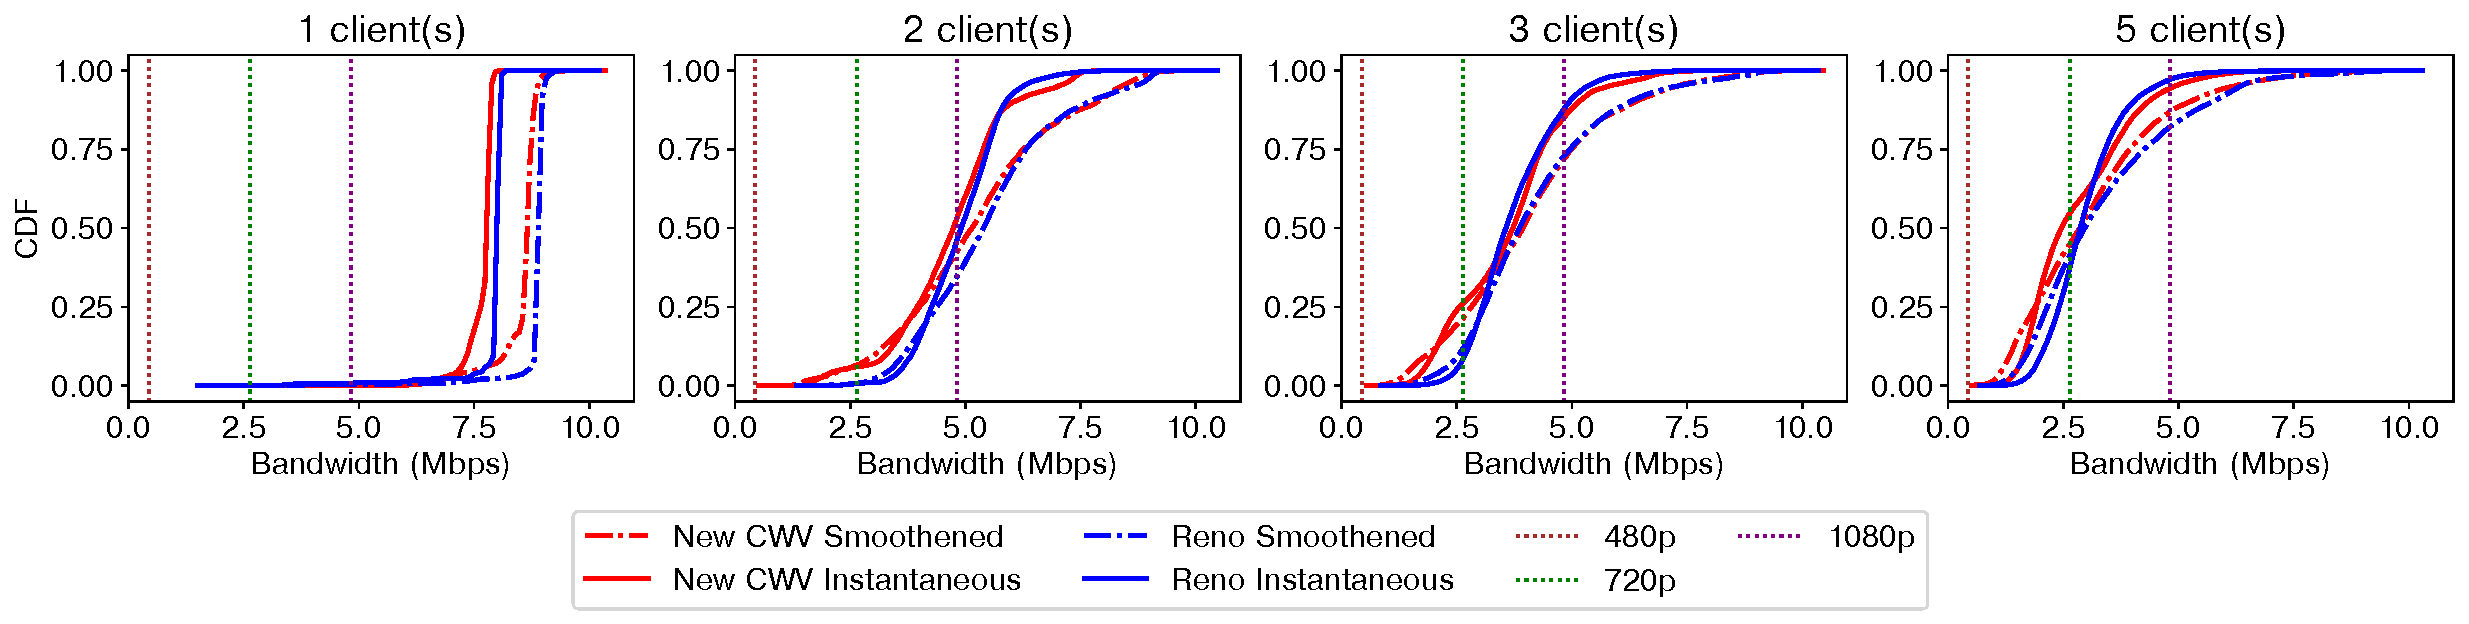
\includegraphics[width=\textwidth]{figures/Throughput_DSL.pdf}
    \label{fig:throughput-clients-DSL}
  }
  \\
  \subfloat[FTTC]{
    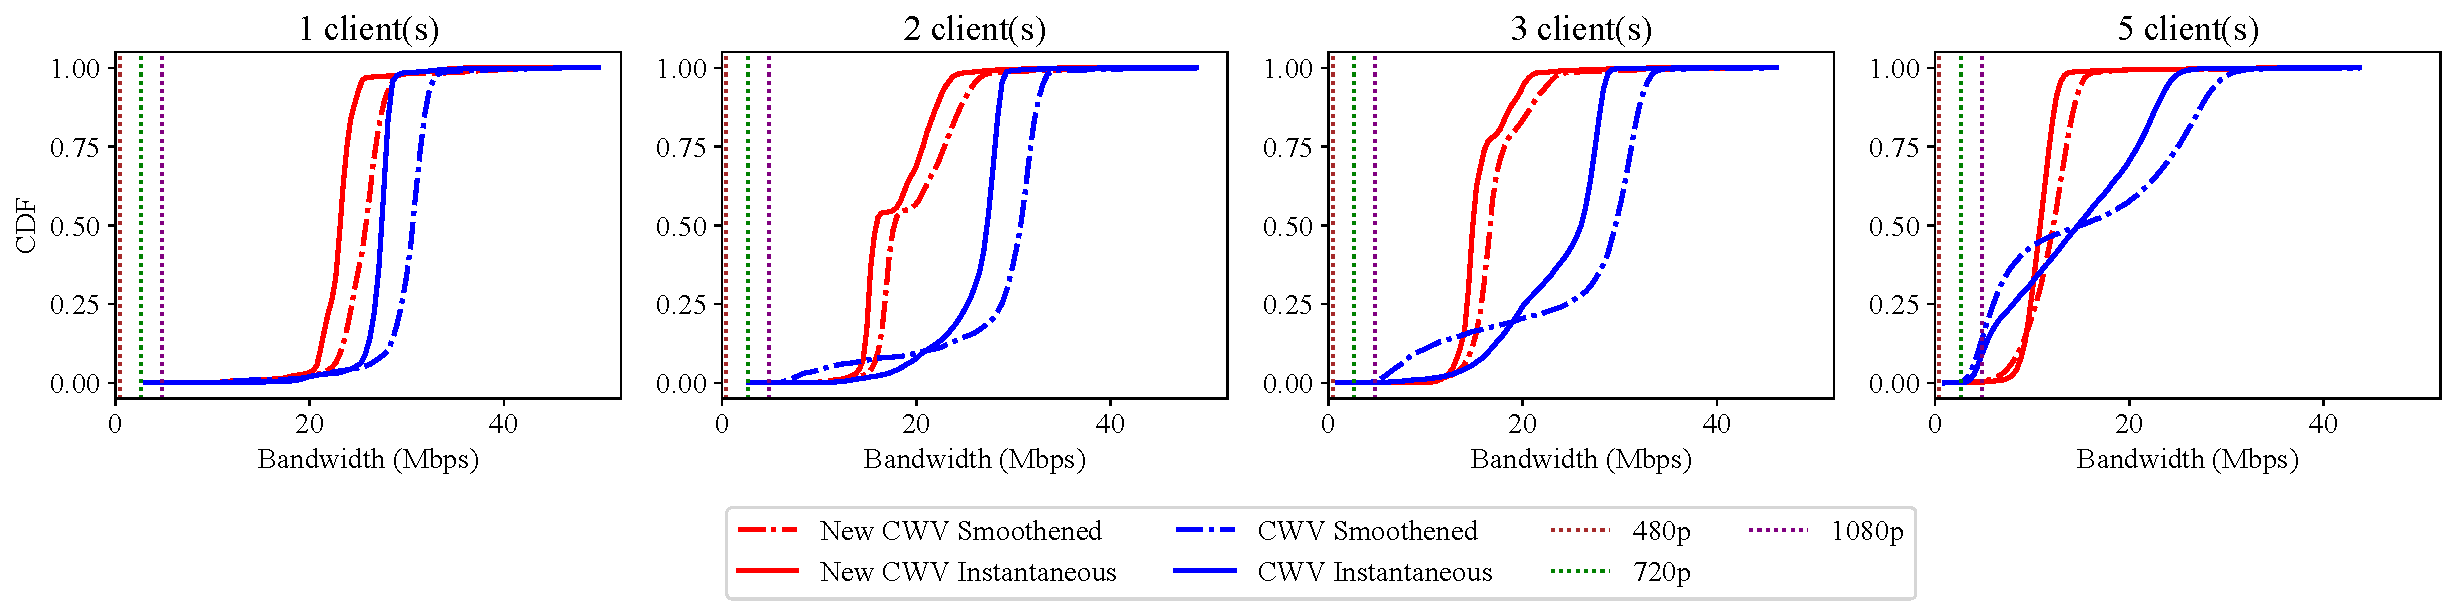
\includegraphics[width=\textwidth]{figures/Throughput_FTTC.pdf}
    \label{fig:throughput-clients-FTTC}
  }
  \caption{dash.js client throughput measurements}
  \label{fig:throughput-clients}
\end{figure*}

Figure~\ref{fig:throughput-clients} shows the cumulative distribution function of all instantaneous and smoothed throughput measurements as seen by the clients. In it, a steep function would indicate that most throughput values have seen little variation, and are therefore highly consistent. 
This is the case for all FTTC cases except the one with one client, where the link capacity was much higher than the highest video representation bandwidth requirement. Because of this high discrepancy the New CWV client could not operate close to the link capacity and therefore could not get an accurate estimation of the available capacity. We note that in reality, presence of cross-traffic is likely to occur and also note that even in this case New CWV's video stability was higher as shown in Section \ref{sec:QoE-impact}. For all other cases, since clients were able to leave slow-start earlier, having less oscillating \emph{cwnd} compared to that of clients using CWV and have expectedly shown a steeper CDF throughput function. 

In addition to being more consistent, 
Clients with New CWV enabled reported estimates that were lower overall. This can be explained by the behaviour of CWV illustrated in Figure~\ref{fig:cwv}: CWV will always reach the maximum link capacity because of its longer slow-start phase. Nazir et al.~\cite{Nazir-2014-performance-evaluation-congestion-window-validation-dash-newcwv}also saw this behaviour. This also supports our initial hypothesis that streaming clients measuring throughput will be able to obtain estimates that are more stable. Finally, as for all client combinations the FTTP link's capacity was much higher than what the highest rate the video clients demanded, both clients with New CWV and CWV showcased similar performance having high stability.

\begin{figure}[t!]
  \centering
  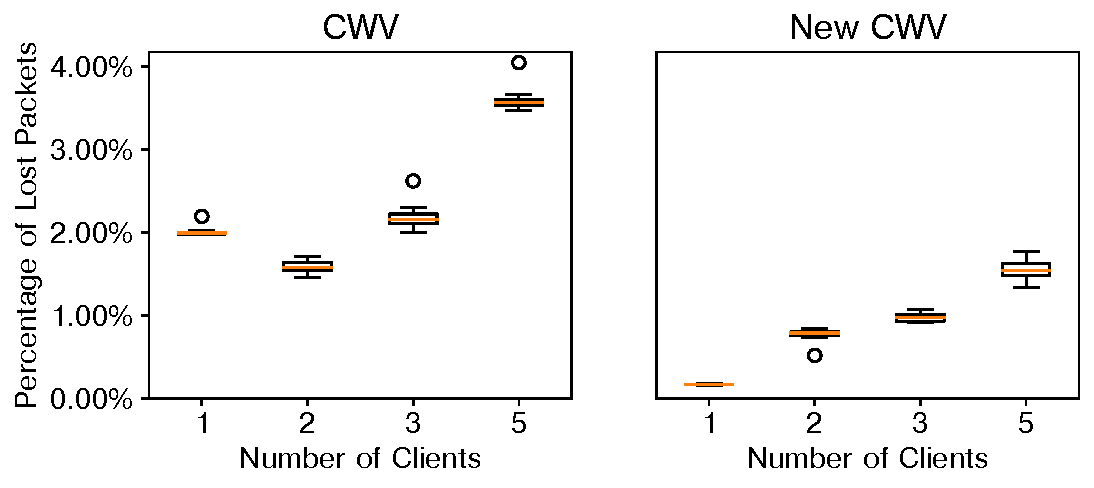
\includegraphics[width=.45\textwidth]{figures/lost_packets.pdf}
  \caption{Lost Packets DSL}
  \label{fig:lost-packets}
\end{figure}

We illustrate the impact of New CWV on packet loss in Figure~\ref{fig:lost-packets}. New CWV consistently achieves lower loss when compared to CWV, with the former having packet loss rates that are up to half of the latter. This confirms our hypothesis for loss and conforms to the description in Section \ref{sec:background}: New CWV exits slow-start earlier, does not overshoot its window, and therefore is able to avoid the loss seen near the end of slow-start that CWV experiences (Figure~\ref{fig:transmission-after-idle}).

The loss values shown here are reported as seen when the \textsc{dynamic} algorithm was used to request video. We have not shown a graph for \textsc{throughput} as well, as we observed that these two algorithms do not make a significant difference with respect to the amount of lost packets.


%--------------------------------------------------------------------------------------------------
\subsection{Impact on Video QoE}
\label{sec:QoE-impact}

\begin{figure*}
  \centering
  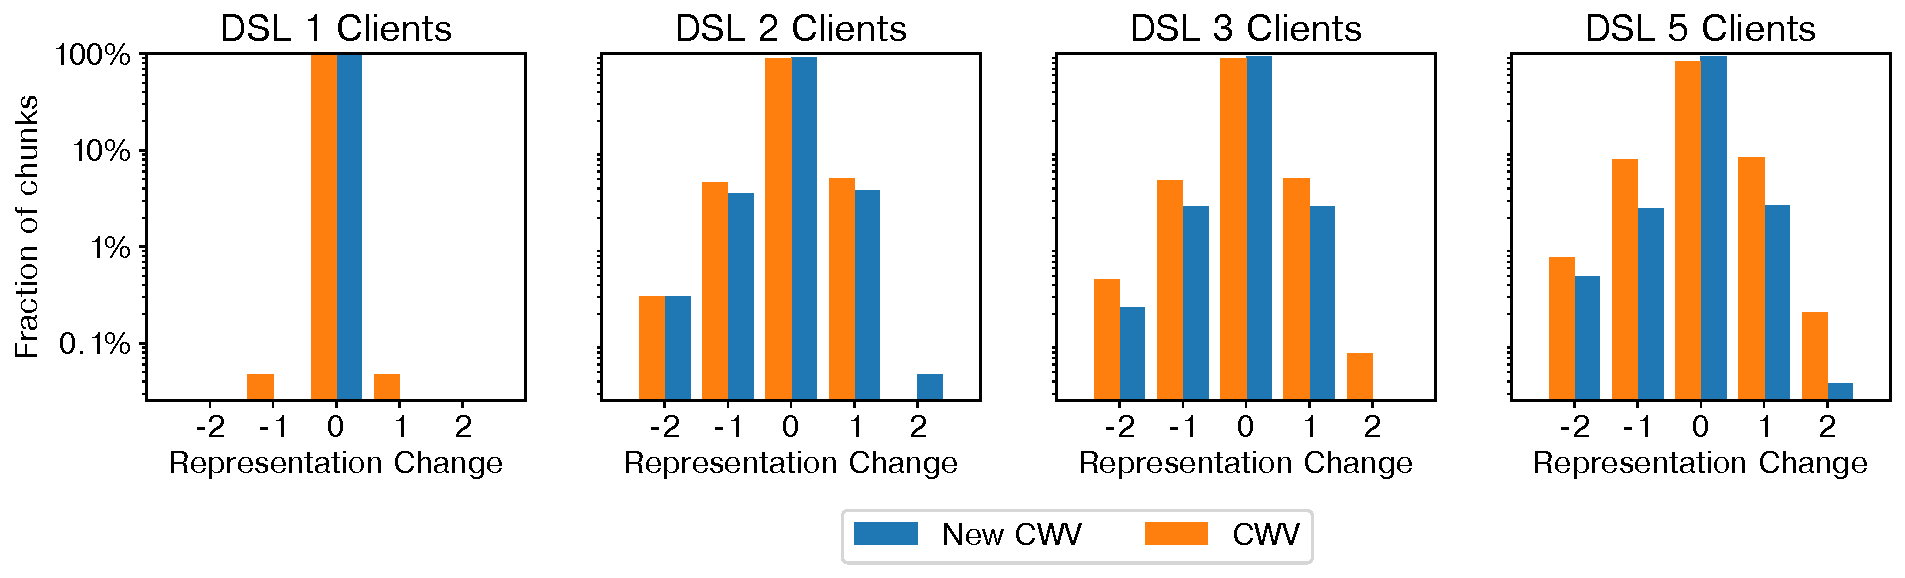
\includegraphics[width=\textwidth, keepaspectratio]{figures/bitrate_derivative_distribution.pdf}
  \caption{Absolute Bitrate Switches (\textsc{throughput})}
  \label{fig:bitrate-switches}
\end{figure*}

\begin{figure*}
  \centering
  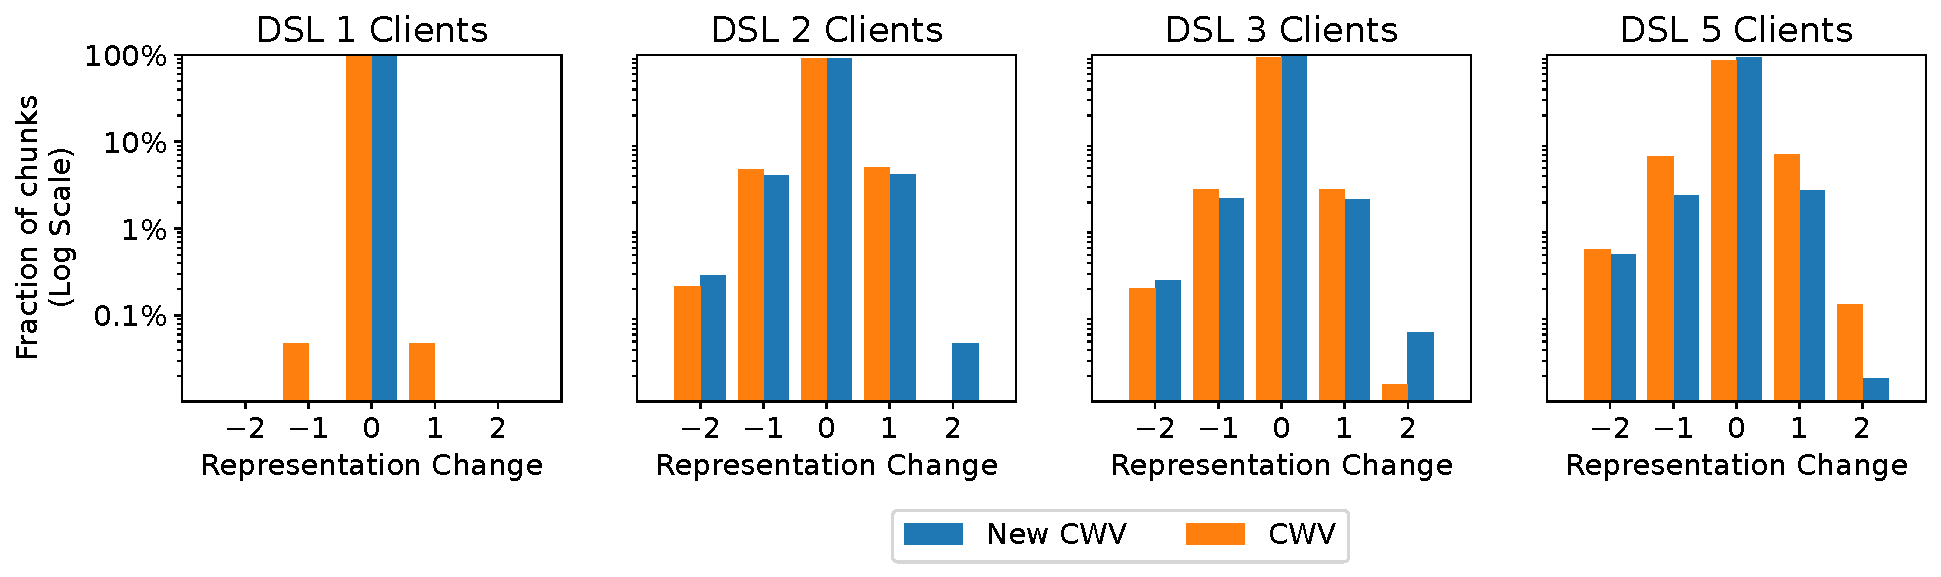
\includegraphics[width=\textwidth, keepaspectratio]{figures/bitrate_derivative_distribution_dynamic.pdf}
  \caption{Absolute Bitrate Switches (\textsc{dynamic})}
  \label{fig:bitrate-switches-dynamic}
\end{figure*}


\begin{figure}
      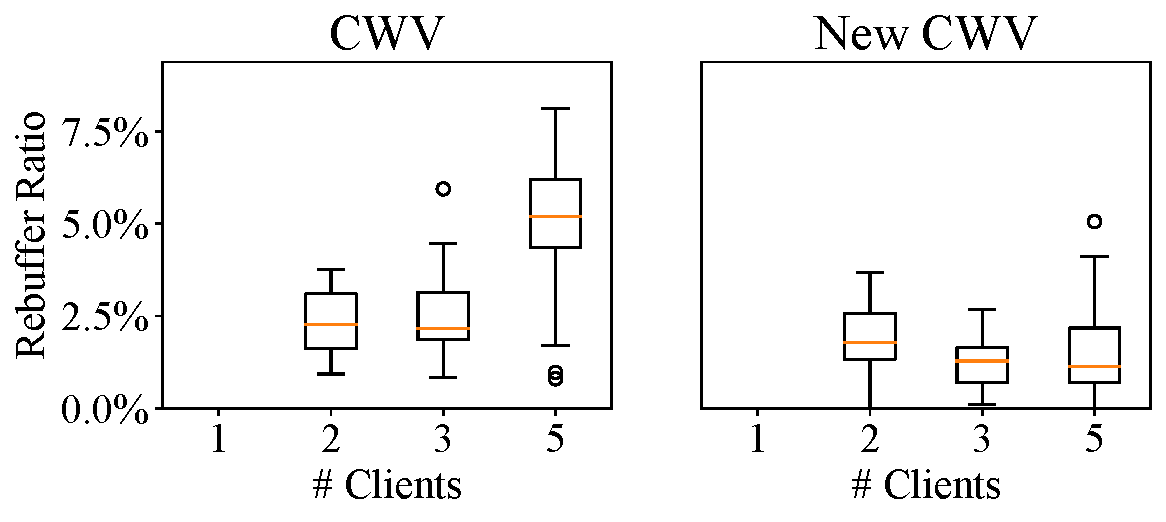
\includegraphics[width=.45\textwidth, keepaspectratio]{figures/Rebuffer_Ratio.pdf}
    \caption{Rebuffer Ratio (\textsc{throughput})}
    \label{fig:rebuffer-ratio}
\end{figure}

\begin{figure}
  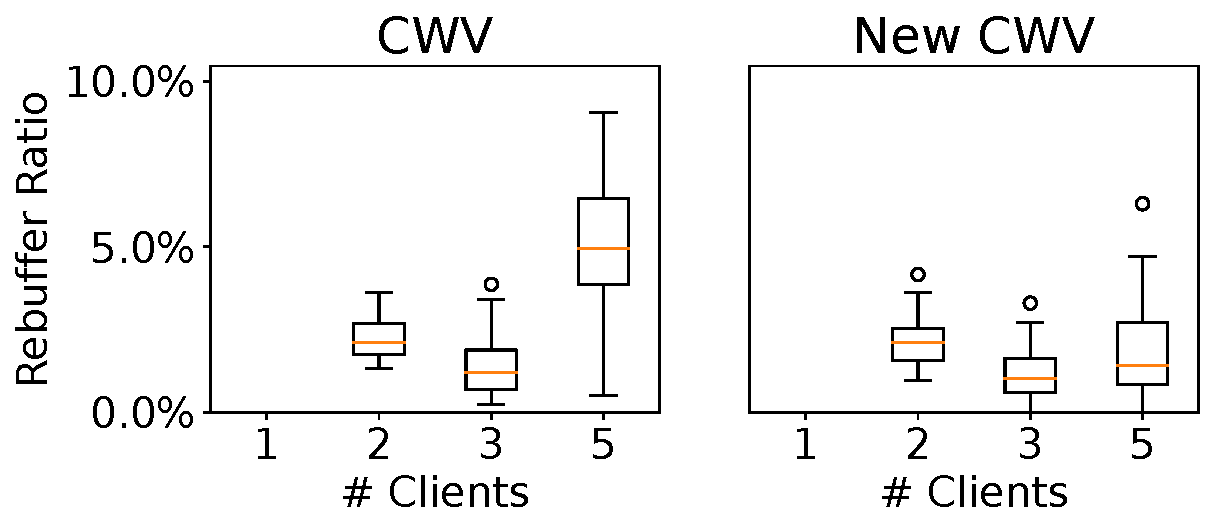
\includegraphics[width=.45\textwidth, keepaspectratio]{figures/Rebuffer_Ratio_dynamic.pdf}
\caption{Rebuffer Ratio (\textsc{dynamic})}
\label{fig:rebuffer-ratio-dynamic}
\end{figure}

To evaluate whether the improved transport layer performance of New CWV translates into improved QoE at the application layer, we report results for the rebuffer ratio and the bitrate switch frequency. We report results for the DSL evaluations, as this link type, in combination with the video encodings used, best highlights the scenario in which New CWV is most beneficial. With FTTP the combination of clients and video encodings enabled all clients to stream at the highest quality without hitting the link limits. This was also the case for all FTTC simulations, with the exception of the 5 client one. In it, we observed a similar pattern as that shown for DSL. We believe that the problem we describe here would be applicable to faster links as applications' network demands increase, f.e., higher video resolutions are seeing more deployment, or as other network-heavy applications start competing for the links' resources (e.g., virtual and augmented reality). Furthermore, we note that the issues we found with the DSL link still have high impact as over 30\% of the households in the UK used a DSLv2 connection or similar in 2019 \cite{ofcom-2020-report}. 

\todo{Make the DSL link case in the last sentence more global and not as UK specific.}

Figure \ref{fig:bitrate-switches} shows the observed bitrate switch distribution using the  \textsc{throughput} algorithm. The proportion of the requested chunks (\emph{y axis}) is shown using a logarithmic scale. The representation change (\emph{x axis}) is the magnitude of the chunk-by-chunk bit rate switches. For example, if a chunk is requested at the same bit rate as the preceding chunk, the difference is zero. If the chunk is of the next higher encoding, compared to its predecessor, the difference is 1, and if it is of the next lower encoding the difference is -1, and so on. We see that for the case with 5 clients, connections with CWV experience non-zero quality switches for 17.4\% of the video duration, compared to 5.7\% for connections with New CWV. For a video consisting of just over 200 chunks, an 11.7 percentage point difference means that, on average, New CWV connections see 24 fewer switches over the course of the video playback.


Comparing Figures~\ref{fig:bitrate-switches} and~\ref{fig:bitrate-switches-dynamic}, we see that when CWV is used, the dynamic algorithm shows a significant improvement in reducing the non-zero representation quality changes. Looking at connections with New CWV, we do not see a significant difference when \textsc{dynamic} was used. This is since New CWV connections had a lower number of non-zero changes even when \textsc{throughput} was used.


Figure \ref{fig:rebuffer-ratio} shows the fraction of the video playback where the connection's media did not progress or otherwise was waiting for more content before it can resume playing, when using the \textsc{throughput} algorithm. The value is shown in percentage relative to the whole media playtime. Again, looking at the 5 client case, we see that New CWV experiences less rebuffering overall. The mean rebuffering values for the 5 client case are 5\% and 1.5\% for CWV and New CWV respectively. For a 10 minute video, this 3.5 percentage point difference accounts for over 21 seconds of rebuffering time.

Figure \ref{fig:rebuffer-ratio-dynamic} shows the fraction of the video playback where the connection's media did not progress or otherwise was waiting for more content before it can resume playing for the \textsc{dynamic}. The value is shown in percentage relative to the whole media playtime. Similar to our discussion on Figure \ref{fig:bitrate-switches-dynamic}, we see that the performance of the connections using CWV has improved, rebuffer-ratio is lower, when \textsc{dynamic} is used. Again, we see that the performance of the New CWV connections does not differ significantly from what was already observed with \textsc{throughput} and is still better than the performance of connections with CWV even in the cases where \textsc{dynamic} was used.

Looking at the average-bitrate, the values reported for connections New CWV and CWV were largely the same. In the rare cases where they differed, New CWV showcased higher video stability \todo{X\% more stable}.


We conclude that New CWV achieves higher video stability when multiple clients are competing on a constrained link, with improved encoding stability and decreased rebuffering time. We have observed this behaviour mainly on the simulated DSL link, since our highest video encoding is just under 5Mbps, however, we note that in practice higher encodings are also used.\footnote{\url{https://support.google.com/youtube/answer/1722171}}

Additionally, we have observed that when New CWV is enabled, the application metrics achieved for connections using either \textsc{dynamic} and \textsc{throughput} are very similar. We observe that a more complex algorithm, such as \textsc{dynamic} has a significant impact on connections with CWV. However, even with an increasingly more complex algorithm at the application layer, the QoE of the CWV connections still lower than the connections with New CWV.

We found that \textsc{dynamic} improved the QoE for connections using CWV, but did not make much difference in the cases where New CWV was enabled. This was due to New CWV connections achieving high QoE, even when \textsc{throughput} was used.

%--------------------------------------------------------------------------------------------------
\subsection{Summary}
\label{sec:summary}

% Compared to \cite{Nazir-2014-performance-evaluation-congestion-window-validation-dash-newcwv} Figure~\ref{fig:throughput-clients} observed similar throughput distribution pattern. We observed lower loss for New CWV connections than they documented. We note that our environment tries to represent a more realistic case for video streaming as of the time of writing this paper. We have reconstructed their environment and used incremental RTT values starting from 40 (the value we used) going to 200 ms (the value they used) in incremental steps of 10 ms. We confirm that as the RTT increases New CWV connections experience higher loss and start to show closer results to when CWV is used. However, even with our incremental RTTs we have not managed to get higher but not as high loss rate as the one reported by the original authors. We attribute this difference to the fact that they used an older version of New Reno and their adaptive algorithm was very different to the current, dash.js, ones. 

We observed that New CWV's more consistent bandwidth measurements (Figure~\ref{fig:throughput-clients}) translate to fewer lost packets (Figure~\ref{fig:lost-packets}), fewer representation switches (Figures \ref{fig:bitrate-switches} \& \ref{fig:bitrate-switches-dynamic}), and lower rebuffering ratio (Figures \ref{fig:rebuffer-ratio} \& \ref{fig:rebuffer-ratio-dynamic}).
This is since the more consistent measurements better match the available network conditions, allowing clients using New CWV to better adapt to the constraints of the bottleneck link. 

The scenarios investigated by this work have used links that emulated a wired
residential Internet connection.  WiFi and cellular links, however, are known
to have very different properties that can affect TCP performance. Understanding
how use of TCP New CWV affects video performance on such links is outside the
scope of this current work.

Our experiments investigated the effects of New CWV on video delivered
using TCP New Reno. This was done to align with
\cite{Nazir-2014-performance-evaluation-congestion-window-validation-dash-newcwv},
and because a recent study \cite{Mishra-2019-the-great-internet-tcp-congestion-control-census}
found New Reno was still widely used for video delivery.
%
TCP Cubic grows its congestion window in slow start using the HyStart++
algorithm \cite{draft-ietf-tcpm-hystartplusplus}, and TCP BBRv2 tracks
bandwidth estimates during slow start, in both cases to avoid the overshoot
problems we discuss in Section \ref{sec:background} and improve stability.
These can potentially benefit from retaining state after idle periods in
the manner of New CWV; exploring this is for future work.

We have constructed a similar environment to \cite{Nazir-2014-performance-evaluation-congestion-window-validation-dash-newcwv} and have conceptually performed the same experiments. However, our environment was built to match the scenarios that could be seen in 2022. Our findings broadly overlapped with theirs, however, comparing both results would not be fair or possible because of the already mentioned differences in the environments. 

%==================================================================================================
\section{Related Work}
\label{sec:related}

New CWV enhances the CWV algorithm~\cite{rfc2861-2000-padhye-congestion-window-validation}.
Both CWV and New CWV attempt to solve the issue of connection resumption after
an idle period in which TCP's view of the network has become stale. While CWV
addresses the issue for bulk, network-limited applications, New CWV improves
the algorithm for rate-limited applications.
\todo{The remainder of this paragraph was unrelated to the paper; reference
instead prior work to improve TCP performance for rate limited applications --
keep it short.}
%   As a result of their changes, both algorithms alter TCP's send rate.
%   Altering the send-rate of TCP should be taken with caution, such that it
%   does not send too fast to cause congestion collapse
%   \cite{Jacobson-1988-congestion-avoidance} but also, to not let other TCP
%   flows have significant effect on their operation (TCP friendliness). The
%   core idea, of altering TCP's sending dynamics, is not new. Building on work
%   by Mathis et al.~\cite{Mathis-1997-the-macroscopic-behavior-tcp} and Padhye
%   et al.~\cite{Padhye-1998-modelling-tcp-throughput}, there has been a
%   significant number of proposals on TCP friendliness and rate
%   control~\cite{rfc-5348-tfrc,Rossi-2010-ledbat,Arun-2018-copa}, including
%   for multimedia~\cite{Carlucci-2016-Analysis-WebRTC,Choi-2007-fairer-tfrc}.
%   These proposals show that it is possible to alter the transport's sending
%   dynamics while remaining friendly to other Internet traffic.

A wide variety of ABR algorithms have been proposed, providing longer-term rate
adaptation to complement TCP dynamics (e.g., \cite{Sun-2016-cs2p,Jiang-2012-improving-fairness-http-video-festive,Spiteri-2016-BOLA,Huang-2015-A-buffer-based-approach-to-rate-adaptation-bba,Spiteri-2019-from-theory-to-practice-sabre,Wang-2016-squad}).
Work on such ABR algorithms has slowed, however, with more recent proposals optimising for specific use cases (e.g., \cite{Karagkioules-2020-achieving-low-latency}), perhaps due to the diminishing improvements obtained \cite{Yin-2015-a-control-theoritic-approach}. We identified cases (e.g., multiple clients competing on a constrained link) where the current state-of-the art algorithms perform poorly, and showed that transport changes, such as enabling New CWV, can have positive QoE impact, with up to 4\% points of improved rebuffering and 12\% points of more stable chunk selection. 
It is difficult to deploy changes to TCP, but the introduction of QUIC \cite{RFC9000}
provides an opportunity to change the transport. QUIC congestion control states that 
New CWV \emph{may} be implemented \cite{RFC9002}; our results suggest it \emph{should}
be implemented when using QUIC with ABR video.

%==================================================================================================
\section{Conclusions}
\label{sec:conclusion}

In this paper, we have shown that enabling New CWV improves video playback stability. We compared video delivery with CWV and New CWV, and validated the results shown by previous work~\cite{Nazir-2014-performance-evaluation-congestion-window-validation-dash-newcwv}. We reported video delivery scenarios using emulated links representative of connections within a country or region, and examined scenarios with different numbers of clients. We found that enabling New CWV, a transport layer change, can improve application layer performance, reducing the number of encoding switches by up to 12\% points and rebuffering time by up to 4\% points. To sum up, we have shown that transport changes are able to improve the application QoE. We have also shown that these transport changes make the transmission more predictable. We believe, that these improvements would allow simple throughput algorithms to compete with the current state of the art that attempts to mask the transport behaviour. In turn, this might remove the need for adaptation algorithm implementers to mask the transport behaviour, and instead allow them to focus on other aspects of the adaptation process. 

Future work might look at the performance of these algorithms under more dynamic environments, for example, if all clients join the session at random times or in the presence of other cross-traffic.


% We believe that with changes to the transport layer, simple, network-reactive, throughput algorithms will be able to perform comparable to other more complex solutions, such as buffer-based or the dynamic algorithms. In turn, this might enable new work in the field to focus on other aspects improving the adaptation process and not to try and mask the transport's behaviour.

%==================================================================================================
%\section{Acknowledgements}

% Acknowledge funding sources.

%==================================================================================================
\bibliographystyle{ACM-Reference-Format}
\bibliography{paper}
%==================================================================================================
% The following information gets written into the PDF file information:
\ifpdf
  \pdfinfo{
    /Title        (Does TCP New Congestion Window Validation Improve HTTP Adaptive Streaming Performance?)
    /Author       (-)
    /Subject      (Video Streaming)
    /Keywords     (TCP, MPEG DASH, Congestion Window Validation)
    /CreationDate (D:20220317130400Z)
    /ModDate      (D:20220317130400Z)
    /Creator      (LaTeX)
    /Producer     (pdfTeX)
  }
  % Suppress unnecessary metadata, to ensure the PDF generated by pdflatex is
  % identical each time it is built. This needs pdfTeX 3.14159265-2.6-1.40.17
  % or later.
  \ifdefined\pdftrailerid
    \pdftrailerid{}
    \pdfsuppressptexinfo=15
  \fi
\fi


%==================================================================================================
\end{document}
% vim: set ts=2 sw=2 tw=75 et ai:
